%!TEX root = ../template.tex
%%%%%%%%%%%%%%%%%%%%%%%%%%%%%%%%%%%%%%%%%%%%%%%%%%%%%%%%%%%%%%%%%%%%
%% chapter4.tex
%% NOVA thesis document file
%%
%% Chapter with lots of dummy text
%%%%%%%%%%%%%%%%%%%%%%%%%%%%%%%%%%%%%%%%%%%%%%%%%%%%%%%%%%%%%%%%%%%%

\typeout{NT FILE chapter4.tex}%

%\glsresetall

\chapter{Results}
\label{cha:results}

\textit{In the following section, the results of the benchmarking study are presented across three main levels: the algorithms, the reference and the query dataset. For each level, the metrics to assess the performance are analyzed to capture both computational feasibility and biological relevance. A final ranking combines all the scores, aiming to identify the best algorithm providing real-world applicability at each dimension of data.}

A full evaluation was conducted with 86 runs (Table~\ref{tab:tablesupplementary1}), resulting from the combination of 10 query datasets and 9 reference datasets (excluding self-comparisons). Given the extensive number of individual runs, the results will be presented as performance summaries of the four key dimensions: algorithms, datasets, reference, and target identification performance. Table~\ref{tab:tablesupplementary1} presents the runs that were evaluated, detailing which combination of query and reference datasets was used, and some characteristics of each query dataset.

\section{Algorithms} % (fold)
\label{sec:algorithmsresults}

To evaluate the performance of the 27 algorithms, several metrics were used describe  the output generated from each package. One is the practical scalability of each tool, and the other is the biological accuracy of the results. To address the first aspect, the scalability (runtime) and the reliability were measured. To evaluate the biological relevance of the predictions, the \gls{AUC}, the win rate, and the pathway enrichment scores were measured.

Execution time and algorithm failures can prevent the use of algorithms in research settings. For this reason, evaluating those metrics is important for understanding the feasibility of each computational approach. The runtime represents the time in seconds that each tool took to execute, and it is directly correlated with query and reference datasets size. In this context, a mean runtime captures how long on average each tool takes to generate the desired output. Whilst this value can be informative, a better approach to present these data is to consider mean runtime per signature (Figure~\ref{fig:fig4.1.algorithmRunTime}) or a value normalized considering the size of the reference dataset (the final runtime score in Figure~\ref{fig:fig4.1.algorithmfinalrankheatmap}). The final runtime score was calculated as follows. First, within each reference, each tool's per-signature times were rescaled from 0 (slower) to 1 (faster). Then, those values were averaged across all references and inverted, so that faster algorithms get higher scores. As shown in Figure~\ref{fig:fig4.1.algorithmfinalrankheatmap}, the majority of topology and enrichment methods topped the rankings with scores greater than 0.90, except for the enrichment methods udt and viper, which had lower scores (0.63 and 0.39, respectively). The topology methods, causal reasoning, interconnectivity, and network propagation, along with the enrichment methods ulm, wmean, and wsum, topped the rank with scores near 1, providing final output on average in 1-2s per signature. Connectivity-mapping tools stayed in the middle of the ranking with scores ranging from 0.80 to 0.90, and mean runtimes ~13-~24s per signature. In contrast, methods like NicheNet and \gls{ProTINA} (respectively 416s and 126s per signature) were markedly slower, thus obtaining a score close to 0.

To complement the runtime evaluation, a reliability score was also computed to assess how often each algorithm failed. The final reliability score is an average of a success rate (runs that returned results) and a run rate (runs launched) from a scale of 0 to 1, where scores close to 1 indicate more reliable algorithms. The rates can be found in Table~\ref{tab:table4.2}, while the final reliability scores are represented in Figure~\ref{fig:fig4.1.algorithmfinalrankheatmap}.At the top of the rank, some of the topology and enrichment methods, with  causalReasoning, randomWalk, and ulm topped scoring close to 0.99 (i.e. returning results in 98\% of the launched runs). Next in the ranking it can be found overconnectivity (score of 0.98) and wmean/wsum (scores of 0.91). Consistent with the runtime, the connectivity methods are in the middle with scores between 0.80 and 0.82, with XCos further down with 0.75. At the bottom of the ranking, NicheNet, which although it achieved total success when launched, only ran in 2 out of 86 runs (run rate of 0.02), resulting in a reliability score of 0.51. The worst performers in this category were \gls{CARNIVAL} (score of 0.06) and \gls{CIE} (score of 0.05), which were skipped or failed in every single run. 

\begin{figure}[htbp]
    \centering
    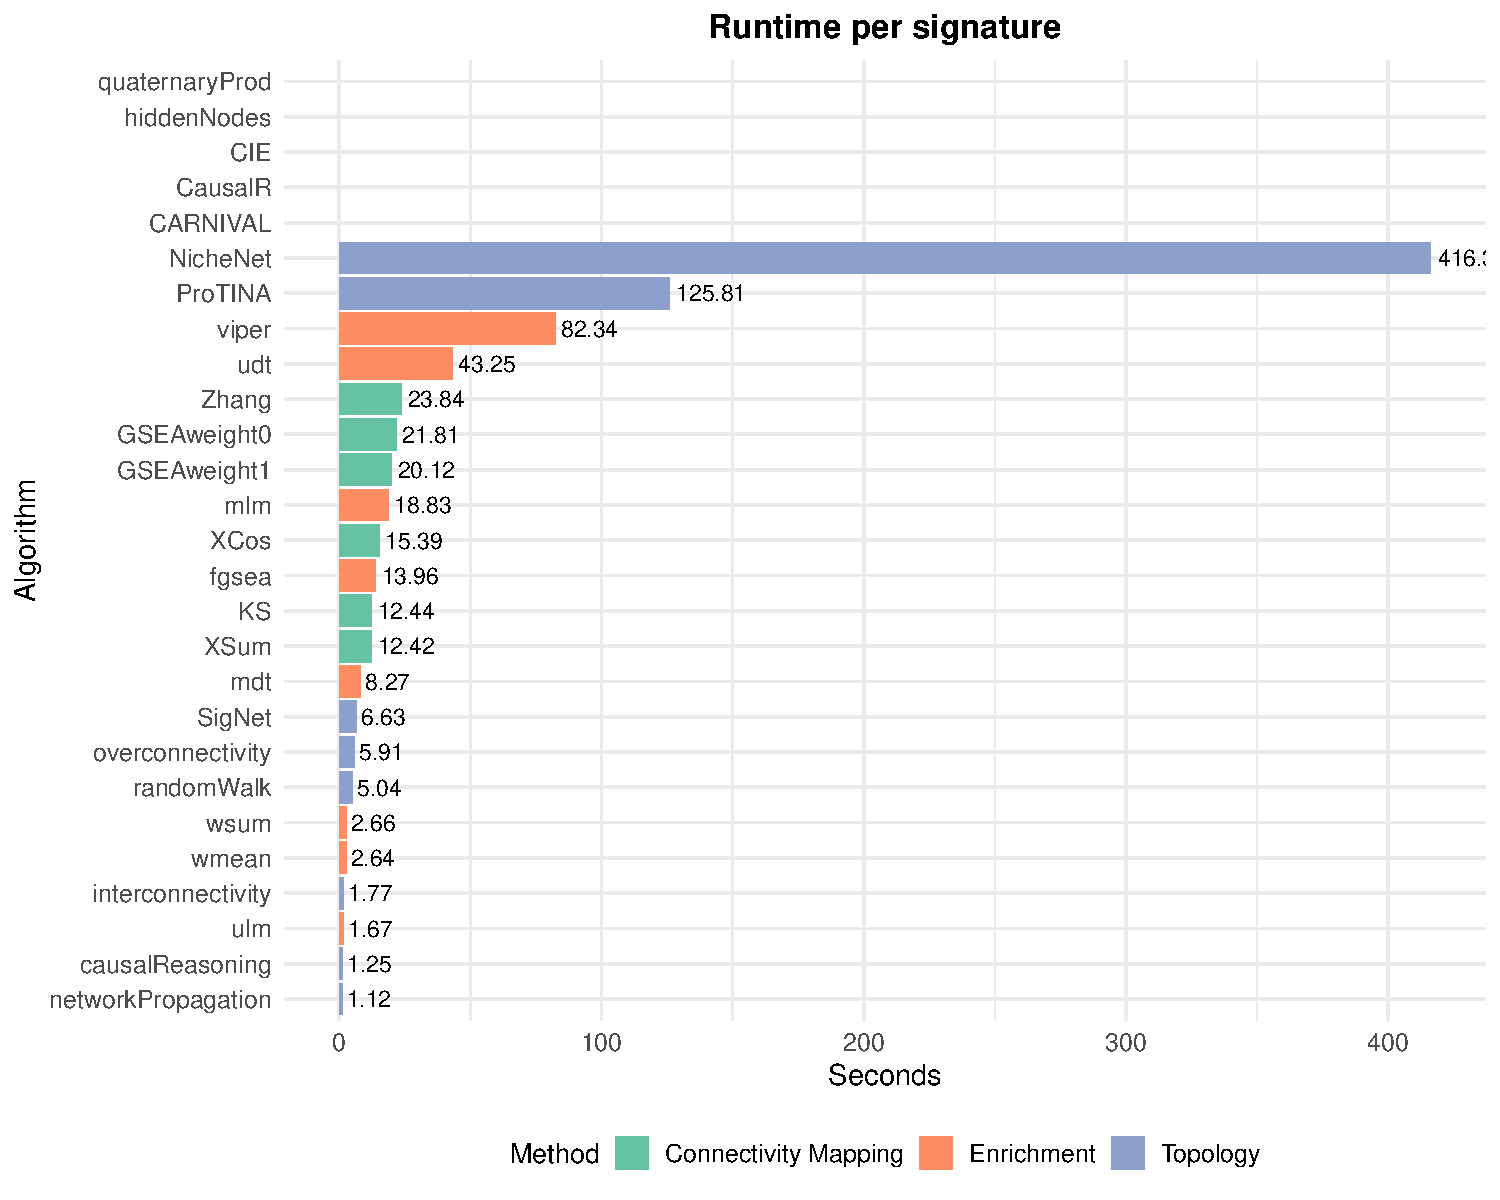
\includegraphics[height=4in]{fig4.1.algorithmRunTime}
    \caption[Runtime per signtures.]{Average runtime per signature in seconds for each algorithm, with values displayed on bars. Algorithms are colored by category.}
    \label{fig:fig4.1.algorithmRunTime}
\end{figure}

The reliability score reflects the capability of providing the designed output. Thus, only the tools that were launched on almost every run and that didn't fail too often, obtained scores close to 1. From a practical point of view, beyond the runtime, reliability is also a critical criterion. Based on these two metrics, \gls{CARNIVAL}, \gls{CIE}, CausalR, hiddenNodes, and quaternaryProd did not complete any benchmarking runs, reflecting their impracticality at this scale. For this reason, these five algorithms were removed from the final evaluation, since they did not behave as expected for a fair evaluation. 

In the research field, only a small number of predictions can be experimentally validated. For that reason, the choice of the algorithms to identify potential target genes should prioritize those that are most likely to include the true target. To evaluate that, the metric area under the recall curve (\gls{AUC}) was used to assess performance in recovering the true target among the top 1\% of the predicted regulators. The \gls{AUC} scaled mean was first calculated by taking the \gls{AUC} mean across all query signatures at the given threshold. Then, for each reference dataset, these means were scaled from 0 to 1 and averaged across all runs for each algorithm. The final \gls{AUC} scores with values close to 1 mean better performance. The mean scaled \gls{AUC} values obtained for each algorithm can be found in Figure~\ref{fig:fig4.1.algorithmAUC}, and the final \gls{AUC} scores in Figure~\ref{fig:fig4.1.algorithmfinalrankheatmap}. 

\begin{table}[]
\caption[Algorithm execution success and run rate across all benchmarking runs.]{Algorithm execution success and run rate across all benchmarking runs. For each of the 24 algorithms evaluated, the number of successful runs, failures, total runs attempted, and runs skipped are reported. Success rate represents the proportion of successful executions among attempted runs (N success / N run). The run rate is the proportion of time where the algorithm was launched ( N total runs / ( N total runs + N skipped ) . Algorithms are ordered by decreasing run rate.}
\label{tab:table4.2}
\begin{tabular}{lllllll}
\hline
\textbf{Algorithm} & \textbf{\begin{tabular}[c]{@{}l@{}}Number\\ success\end{tabular}} & \textbf{\begin{tabular}[c]{@{}l@{}}Number\\ fail\end{tabular}} & \textbf{\begin{tabular}[c]{@{}l@{}}Number\\ run\end{tabular}} & \textbf{\begin{tabular}[c]{@{}l@{}}Number\\ skipped\end{tabular}} & \textbf{\begin{tabular}[c]{@{}l@{}}Success\\ rate\end{tabular}} & \textbf{\begin{tabular}[c]{@{}l@{}}Run \\ rate\end{tabular}} \\ \hline
causalReasoning & 84 & 2 & 86 & 0 & 0.98 & 1.00 \\
randomWalk & 84 & 2 & 86 & 0 & 0.98 & 1.00 \\
ulm & 51 & 1 & 52 & 0 & 0.98 & 1.00 \\
overconnectivity & 83 & 0 & 83 & 3 & 1.00 & 0.97 \\
wsum & 43 & 7 & 50 & 2 & 0.86 & 0.96 \\
wmean & 43 & 8 & 51 & 1 & 0.84 & 0.98 \\
SigNet & 60 & 18 & 78 & 8 & 0.77 & 0.91 \\
KS & 23 & 0 & 23 & 13 & 1.00 & 0.64 \\
GSEAweight0 & 22 & 1 & 23 & 13 & 0.96 & 0.64 \\
GSEAweight1 & 22 & 1 & 23 & 13 & 0.96 & 0.64 \\
XSum & 22 & 1 & 23 & 13 & 0.96 & 0.64 \\
Zhang & 22 & 1 & 23 & 13 & 0.96 & 0.64 \\
udt & 30 & 1 & 31 & 21 & 0.97 & 0.60 \\
interconnectivity & 47 & 0 & 47 & 39 & 1.00 & 0.55 \\
networkPropagation & 47 & 0 & 47 & 39 & 1.00 & 0.55 \\
mdt & 29 & 2 & 31 & 21 & 0.94 & 0.60 \\
XCos & 20 & 3 & 23 & 13 & 0.87 & 0.64 \\
viper & 20 & 4 & 24 & 28 & 0.83 & 0.46 \\
fgsea & 13 & 3 & 16 & 36 & 0.81 & 0.31 \\
NicheNet & 2 & 0 & 2 & 84 & 1.00 & 0.02 \\
mlm & 8 & 6 & 14 & 38 & 0.57 & 0.27 \\
CARNIVAL & 0 & 10 & 10 & 76 & 0.00 & 0.12 \\
CIE & 0 & 9 & 9 & 77 & 0.00 & 0.10 \\
ProTINA & 0 & 0 & 0 & 66 & - & 0.00 \\ \hline
\end{tabular}
\end{table}

\begin{figure}[htbp]
    \centering
    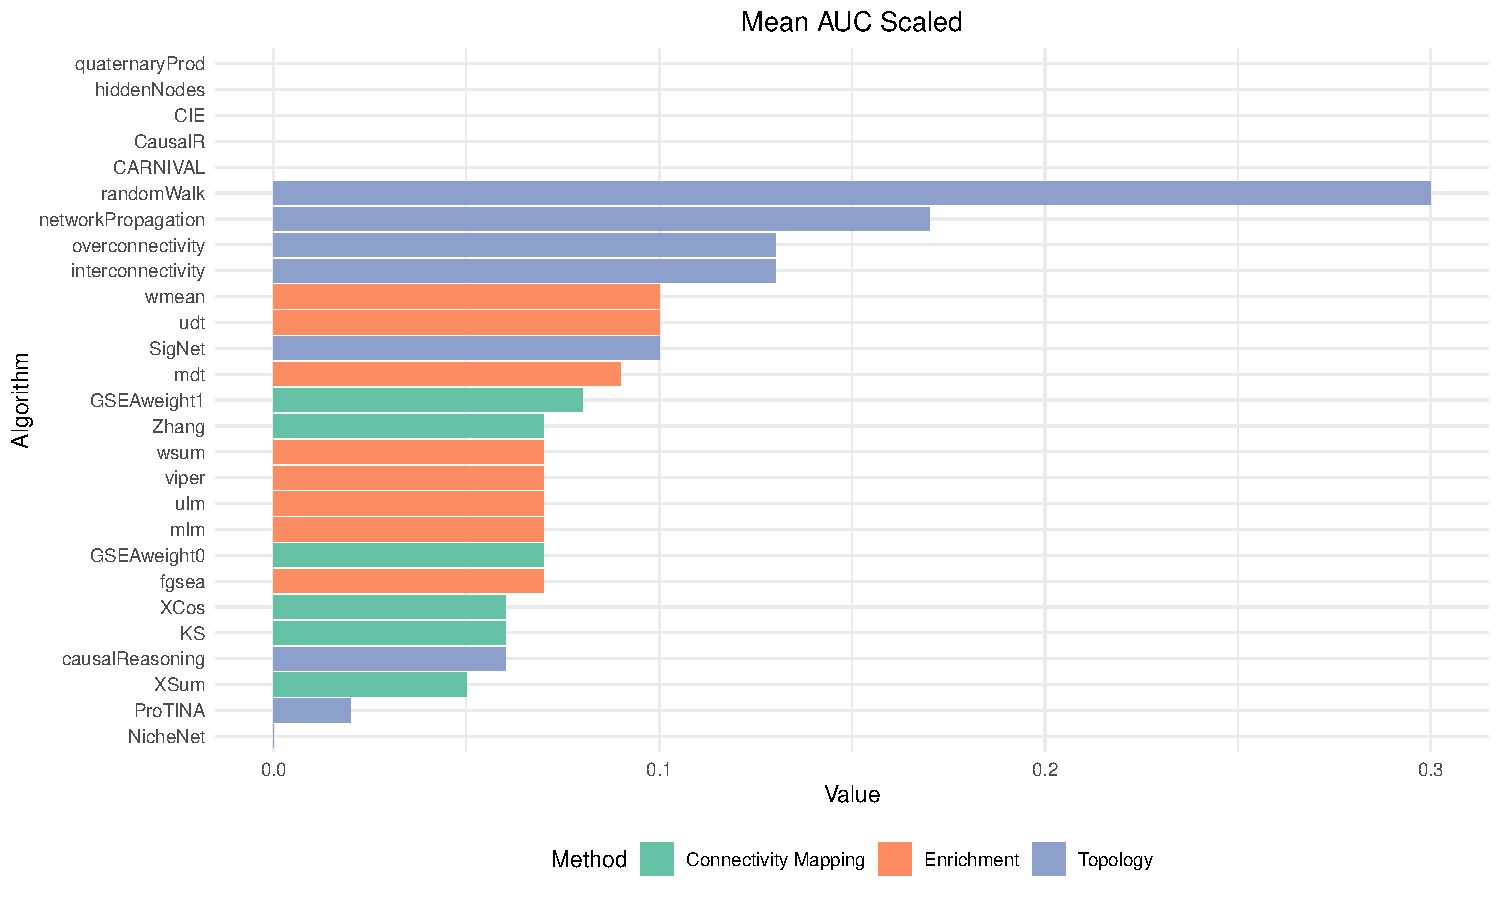
\includegraphics[height=3in]{fig4.1.algorithmAUC}
    \caption[Mean scaled \gls{AUC} values for each algorithm.]{Mean scaled \gls{AUC} values for each algorithm, ordered by performance. Algorithms are colored by category.}
    \label{fig:fig4.1.algorithmAUC}
\end{figure}
%\end{newpdflayout}

The topology-based algorithms with node prioritization occupied the top of the rank, with randomWalk showing the best performance with a mean scaled \gls{AUC} of 0.30 (score of 1), achieving 30\% recovery within the top 1\% of predictions. The others (networkPropagation, interconnectivity and overconnectivity), although at the top, only achieved half the performance of the randomWalk (scaled \gls{AUC} of 0.17, 0.13 and 0.13, respectively). The enrichment-based methods displayed a uniform performance, with scaled \gls{AUC} values clustering between 0.07 and 0.10. Connectivity mapping approaches do not seem suitable for this task, with all five methods achieving scaled \gls{AUC} values below 0.08. The XSum method performed worst overall (scaled \gls{AUC}: 0.05, score: 0.16), while GSEAweight1 represented the best among connectivity tools but still achieved only 28\% of randomWalk's performance. These results suggest that methods designed for perturbation signature matching lack the mechanistic reasoning necessary for an accurate target identification.

The \gls{WPAE} were two metrics used to evaluate how often an algorithm ranks the true targets and the performance over a random selection of target genes. A win rate of 0.5 means that out of 25 different query datasets, the true target is ranked among the top regulators in 25 of them. The \gls{WPAE} is a normalization, to account for a different number of competing tools in different runs. 

A Positive \gls{WPAE} means that the performance was better than chance, and a negative indicates an underperformance of the tool compared to a random selection of target genes. The results of these metrics are shown in Figure~\ref{fig:fig4.3.WinandWPAE}. The randomWalk algorithm stood out with a win rate of 0.29 and a \gls{WPAE} of 0.14. This means it identified the real target more often than the other tools and also above what would be expected by chance. Only two other topology-based methods achieved positive WPAE values, overconnectivity (win rate: 0.17, WPAE: 0.02) and interconnectivity (win rate: 0.14\%, \gls{WPAE}: 0.02).  Most algorithms (19 out of 22) showed negative \gls{WPAE} values, indicating they win less frequently than random chance would predict, revealing that the other approaches rarely identify the true target. NetworkPropagation, despite showing a good \gls{AUC} performance, achieved a slightly negative \gls{WPAE} (-0.05), and won only 8\% of comparisons. This discrepancy suggests the algorithm excels at enriching true targets within its top predictions, but rarely ranks them at the absolute top position.
The win rate score (Figure~\ref{fig:fig4.1.algorithmfinalrankheatmap}) close to 1 for randomWalk (calculated as mean \gls{WPAE} rescaled between 0 and 1), reinforce the superiority of this approach against the other comparators considered.

% In~\ref{fig:fig4.1.algorithmwin}

% In~\ref{fig:fig4.1.algorithmWPAE}

\begin{figure}[htbp]
  \centering
  \subbottom[\label{fig:fig4.1.algorithmwin}]{%
    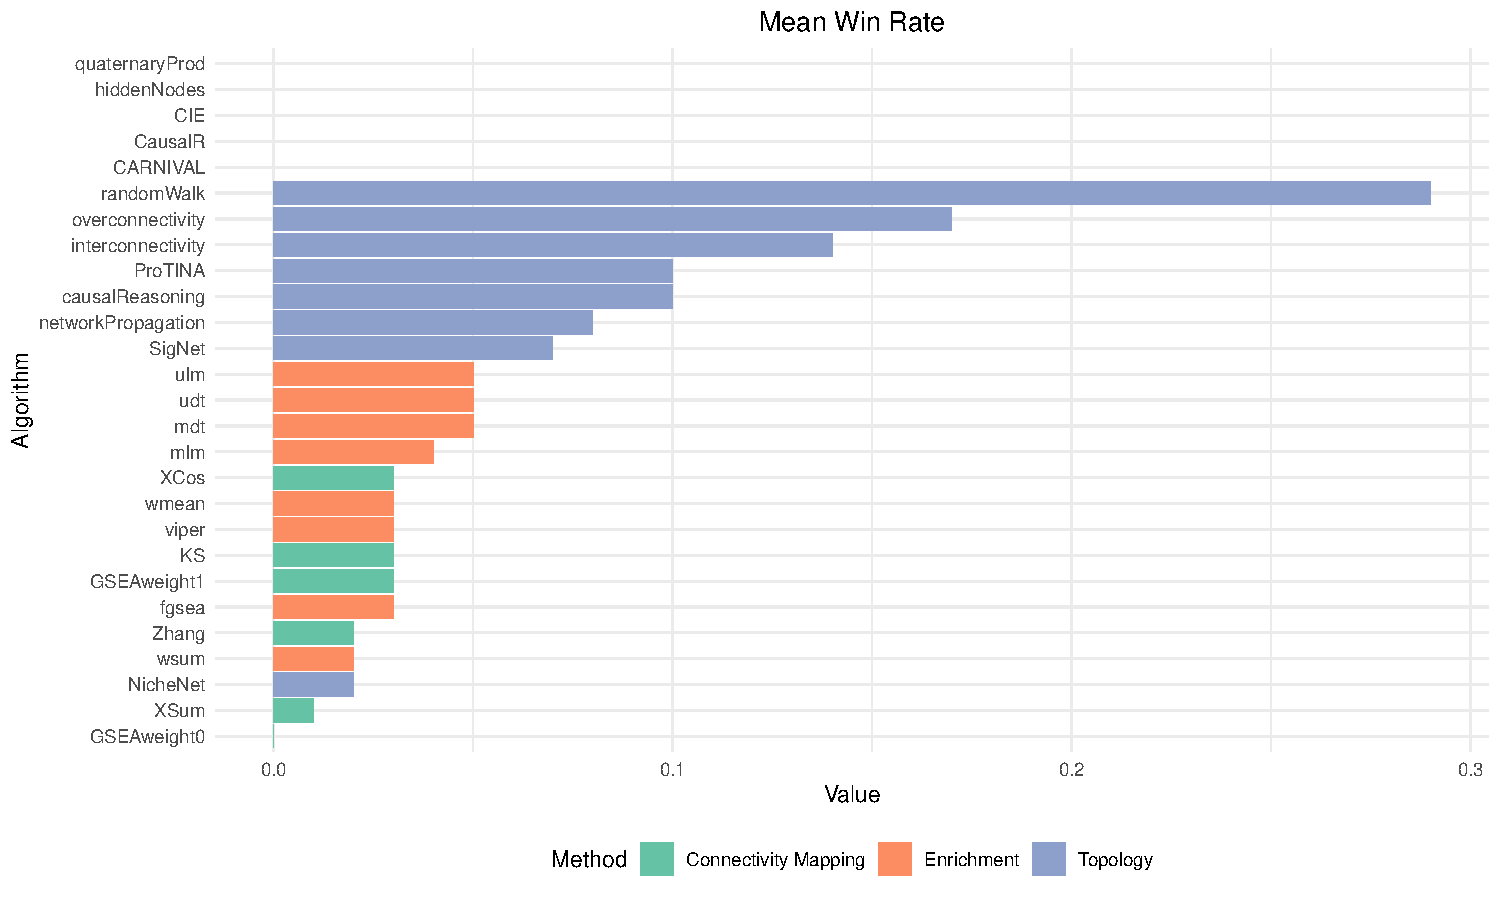
\includegraphics[width=0.5\linewidth]{fig4.1.algorithmwin}}%
  \subbottom[\label{fig:fig4.1.algorithmWPAE}]{%
    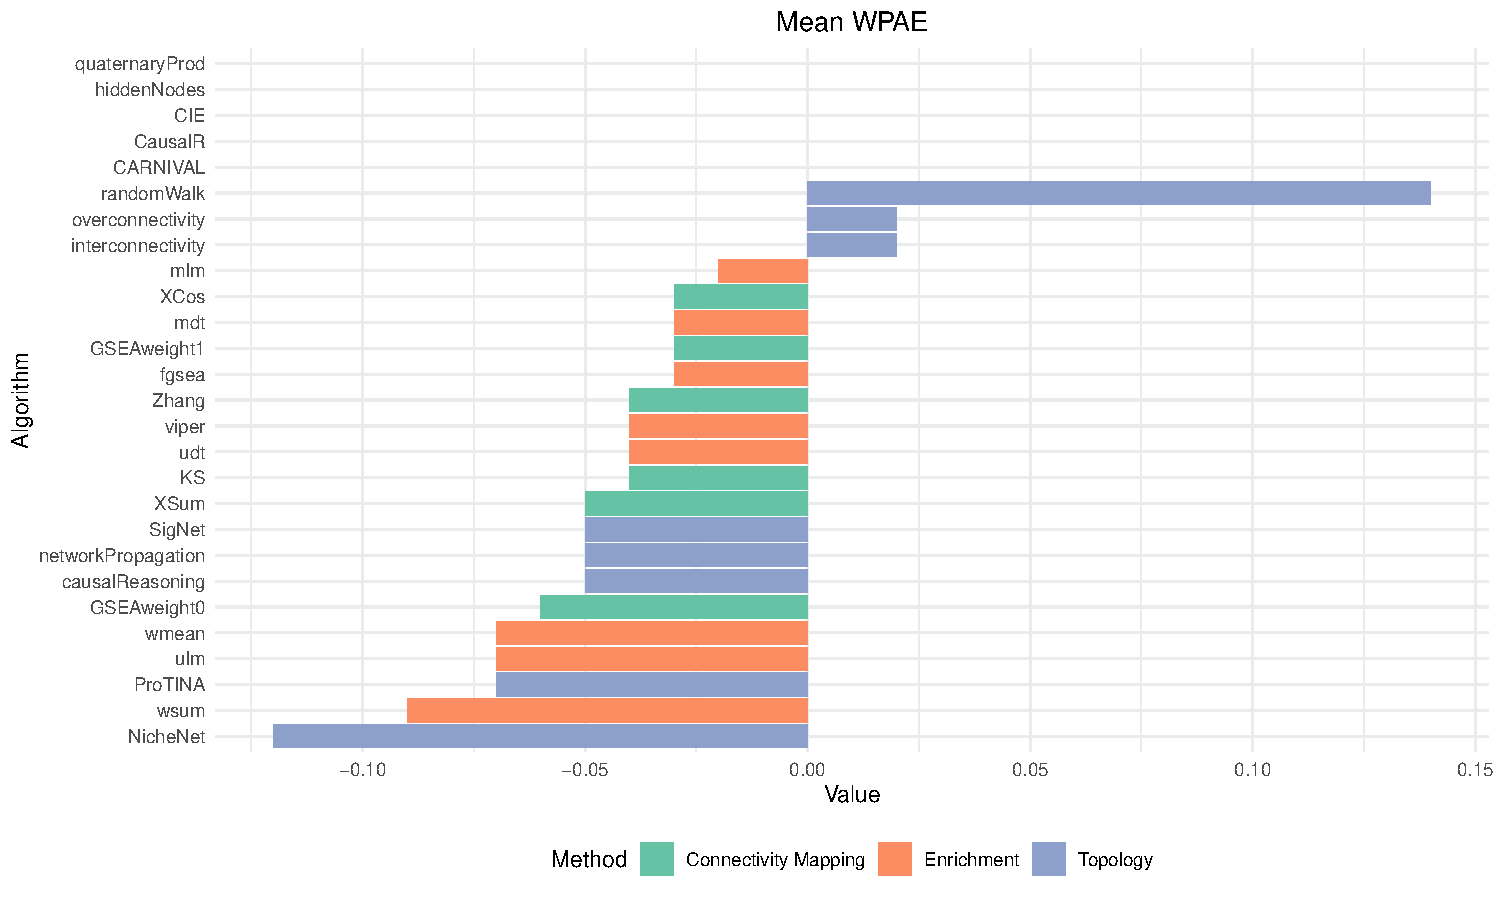
\includegraphics[width=0.5\linewidth]{fig4.1.algorithmWPAE}}%
  \caption[Mean win rate and WPAE across all evaluations for each algorithm.]{A. Mean win rate across all evaluations for each algorithm, showing the frequency of ranking the true target highest among competing methods. B. Mean \gls{WPAE} for each algorithm, showing performance relative to random chance. Algorithms are colored by category.}
  \label{fig:fig4.3.WinandWPAE}
\end{figure}

The mean pathway enrichment (Figure~\ref{fig:fig4.1.algorithmpath}) assesses whether the regulators identified by each algorithm are biologically meaningful. This metric is not evaluating direct target recovery, but rather the ability to identify regulators that are functionally related to the target. Hence, an algorithm with a high pathway enrichment performance should identify a high number of regulators that are enriched in the same pathways as the true target. The pathway enrichment scores (Figure~\ref{fig:fig4.1.algorithmfinalrankheatmap}) are a rescaled mean pathway enrichment metric across all runs, with values closer to 1 indicating higher levels of recovery of target-related pathways. Pathway enrichment performance display interesting patterns when compared with direct target recovery. Enrichment-based methods, which showed moderate performance in direct target recovery, demonstrated an improvement in pathway-level performance. The wmean and wsum methods achieved the best pathway scores (1.00), with average enrichment values of 2.15. This is confirmed by a low hypergeometric p-value, showing a strong overlap between the target pathways and the pathways enriched in the significant regulators predicted by the algorithm. The ulm follows with a mean enrichment of 1.98 (score of 0.92). In contrast to these are viper, mlm, fgsea, mdt, and udt, which performed poorly with values between 1 and 0.24 (scores between 0.45 and 0.08), respectively. Within topology-based methods, causalReasoning achieved the second-highest overall performance (enrichment: 1.97, score: 0.91), followed by overconnectivity (enrichment: 1.72, score: 0.79). Similar moderate performance was shows by networkPropagation, SigNet, and randomWalk (scores in the 0.54 - 0.55 range). Connectivity mapping approaches uniformly failed at pathway enrichment, with all five methods achieving scores below 0.11.

\begin{figure}[htbp]
    \centering
    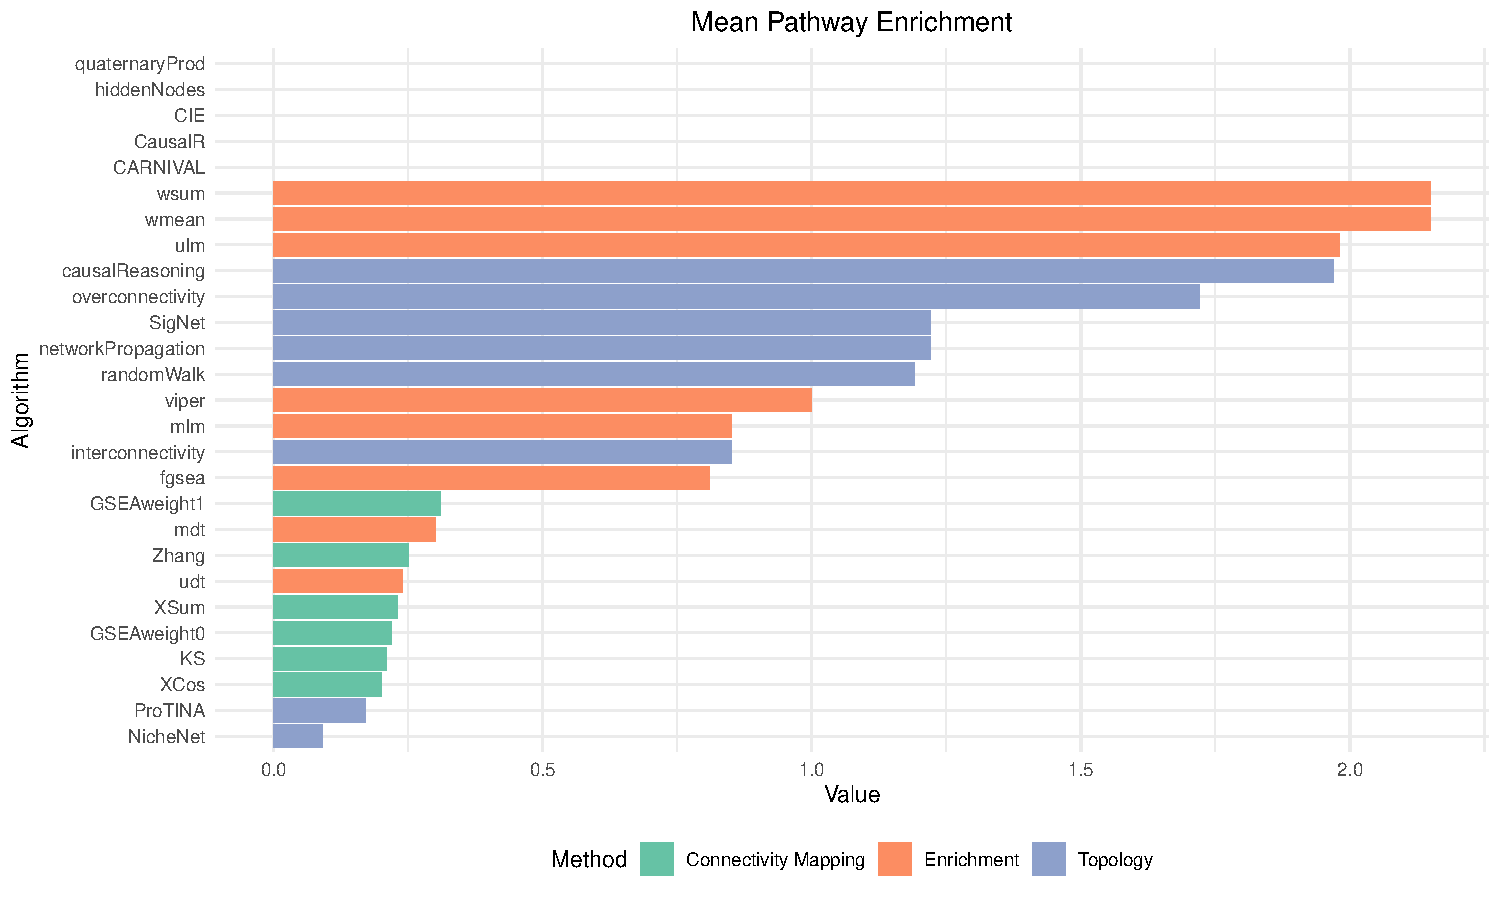
\includegraphics[height=3in]{fig4.1.algorithmpath}
    \caption[Mean pathway enrichment values for each algorithm.]{Mean pathway enrichment values for each algorithm, indicating the ability to identify biologically relevant pathways containing the true targets. Algorithms are colored by category.}
    \label{fig:fig4.1.algorithmpath}
\end{figure}
%\end{newpdflayout}


The outperformance of some of the algorithms in this benchmark should be kept in mind when selecting the best computation approach to understand broad biological context rather than simply identifying single causal nodes. 

\begin{figure}[htbp]
    \centering
    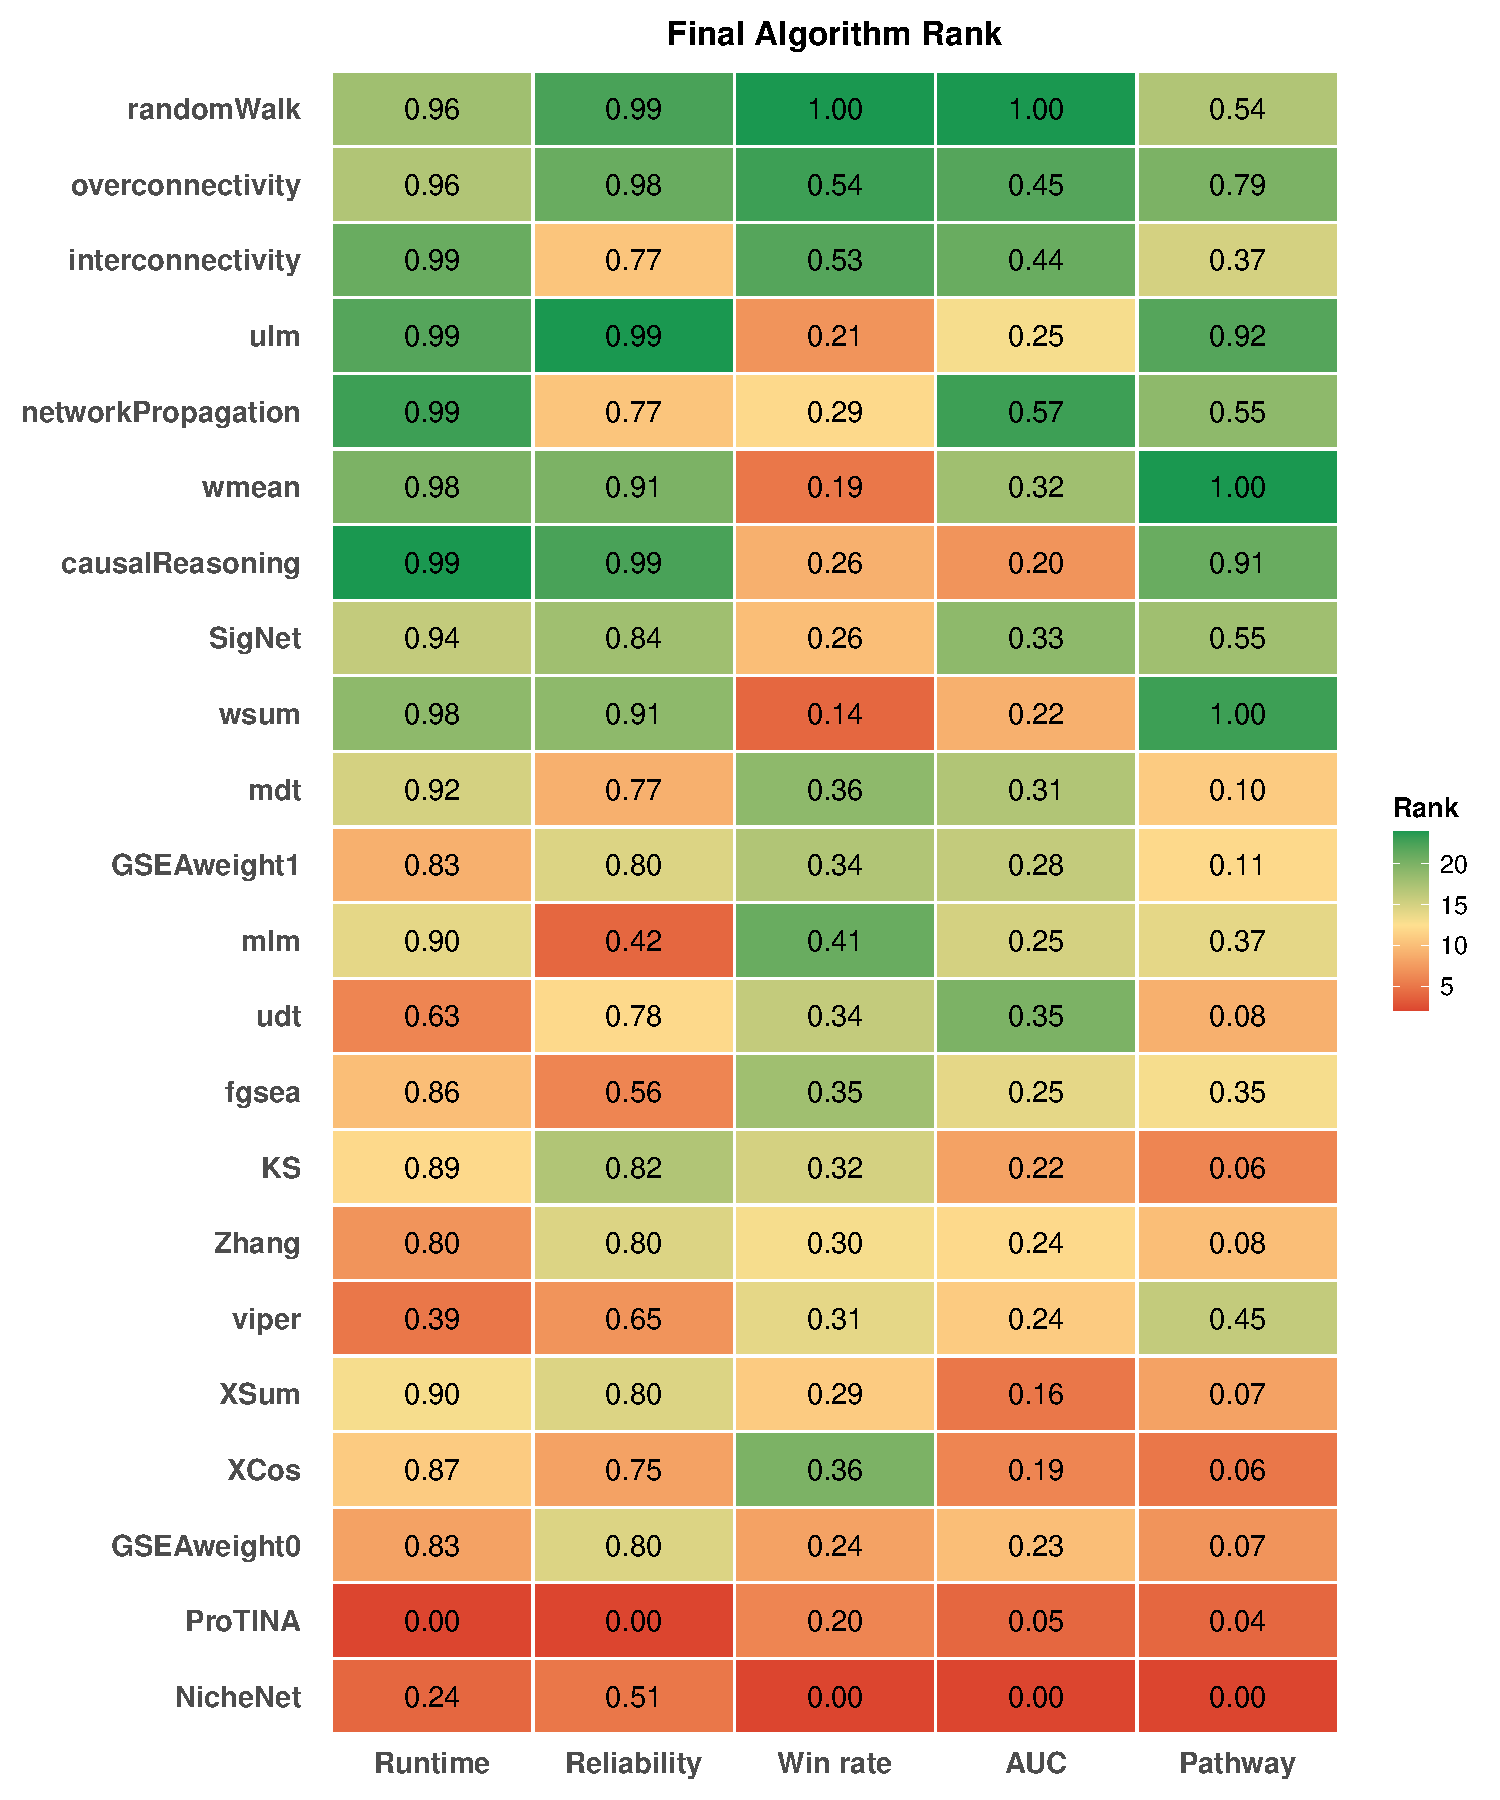
\includegraphics[height=4in]{fig4.1.algorithmfinalrankheatmap}
    \caption[Final performance evaluation of 22 algorithms across five metrics.]{Final performance evaluation of 22 algorithms across five metrics. Heatmap showing algorithm performance rankings, where higher values indicate better performance. Algorithms (rows) are ordered by their final aggregate rank from best (top) to worst (bottom). Each cell displays the normalized performance score (0-1 scale) for the corresponding algorithm-metric combination, with cell colors representing the rank (1-24). The color gradient ranges from red (low rank/poor performance) through yellow (medium performance) to green (high rank/excellent performance). }
    \label{fig:fig4.1.algorithmfinalrankheatmap}
\end{figure}
%\end{newpdflayout}


%%% sUB SECTION: REFERENCE DATASETS
\section{Reference datasets} % (fold)
\label{sec:referencedatasetsresults}

Assessing the influence of other components on algorithm performance is also important. In order to obtain biologically relevant results it is important not only the choice of the algorithm but also the type of prior knowledge used for running the algorithm. For this reason, the nine reference datasets were evaluated to understand which allows more effective recovery of targets identified from the golden standard. As before, four metrics were used to evaluate performance: coverage, win rate, target recovery, and pathway enrichment. For each reference dataset, the metric values and the final rank, with the final scores (values rescaled from 0 to 1) are represented in Figure~\ref{fig:fig4.2.referencewrapplots}. Evaluating the degree of coverage is crucial because if targets are not present in the prior knowledge provided to the algorithm, then they will never be returned in the results. Looking at the broader picture, Figure~\ref{fig:fig4.2.referencewrapplots} shows the weight of the coverage in the final rank, which again highlight the importance of having well annotated and detailed prior knowledge. Overall, the MetaBase network was the best reference dataset. MetaBase network achieved the top rank in both coverage (92\% of targets are present) and target recovery (\gls{AUC} score of 1). OmniPath network ranked immediately next, given the substantial differences in coverage (63\%).  However, it has the highest win rate (and a \gls{WPAE} of 0.05) and pathway enrichment scores, suggesting that the quality of annotation can balance the possible lack of specific regulators. For MetaBase network, the coverage is in line with the number of regulatory interactions present in this database, ensuring that no causal regulators are missed because of lack in the prior knowledge dataset. What stands out most when considering performance of different reference datasets is the fact that topological network references generally score higher than signatures. Also, the clear contrast between MetaBase Network's 92\% coverage and \gls{GWPS}'s 27\% coverage directly translates to the performance differences across all other metrics evaluated. \gls{GWPS} achieved a score of zero in all metrics, showing that even sophisticated algorithms cannot overcome insufficient molecular coverage in a prior knowledge reference data set. \gls{LINCS} \gls{CRISPR} performed best among perturbation references, but scored poorly in pathway enrichment (0.50), indicating that perturbation signatures may lack pathway-level context. Finally, it is worth to mention that the performance of regulon-based references. MetaBase Linear Path Regulons achieved the best pathway enrichment (score of 1) in contrast with the poor coverage (48\%) and target recovery (\gls{AUC}: 0.18). This can indicate that although this dataset captures well the biological context, it probably oversimplifies the complexity needed for precise target identification.

\begin{figure}[htbp]
    \centering
    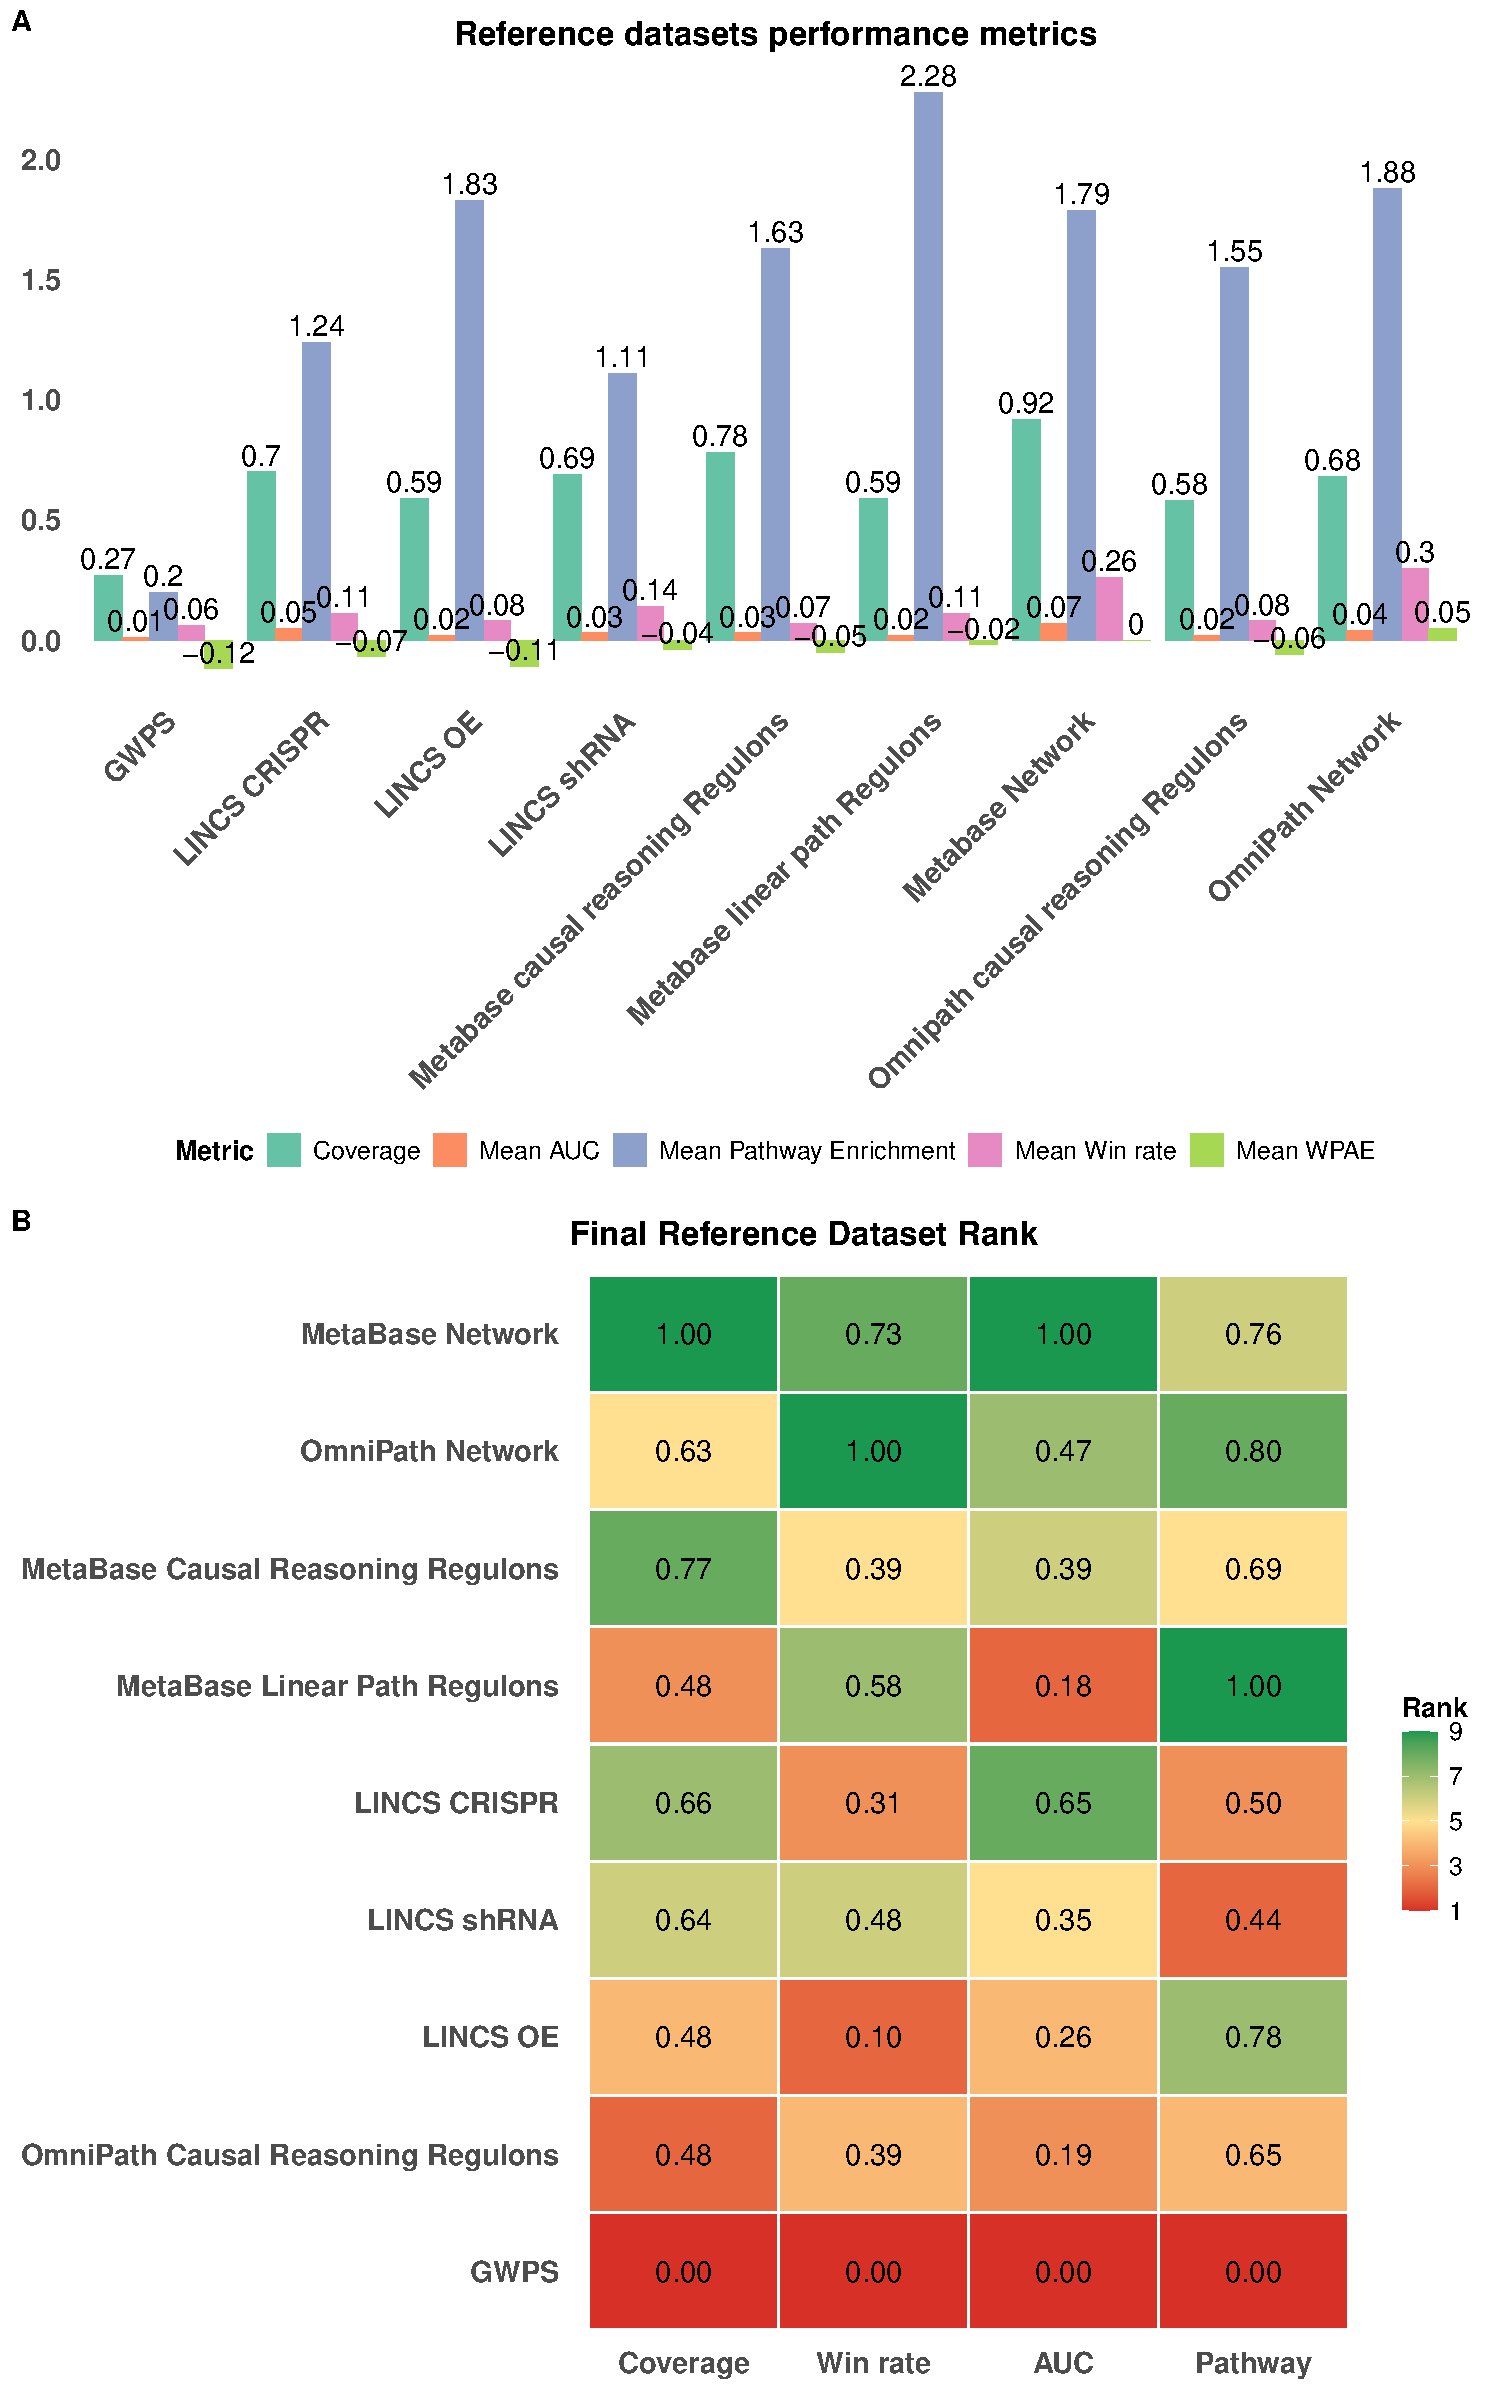
\includegraphics[height=6in]{fig4.2.referencewrapplots}
    \caption[Performance of nine reference datasets across four evaluation metrics.]{Performance of nine reference datasets across four evaluation metrics. A. Performance mean values. For each reference dataset, the performance is colored by metric. The mean pathway enrichment values represent the significance of overlap between true target pathways and pathways enriched with significant regulators ($-\log_{10}(\text{p-value})$ of the hypergeometric test) averaged across the signatures where true targets are present in one or more MetaBase pathways. B. Performance ranking with final scores. Heatmap showing reference dataset performance rankings, where higher ranks indicate better performance. Reference datasets (rows) are ordered by their final aggregate rank from best (top) to worst (bottom). Each cell displays the scaled performance score for the corresponding dataset-metric combination, with cell colors representing the rank. The evaluation metrics include Coverage, Win rate, \gls{AUC}, and Pathway Enrichment. The color gradient ranges from red (low rank/poor performance) through yellow (medium performance) to green (high rank/excellent performance).}
    \label{fig:fig4.2.referencewrapplots}
\end{figure}
%\end{newpdflayout}

\section{Query datasets} % (fold)
\label{sec:querydatasetsresults}

It is essential to comprehend the performance of all components used in computational algorithms, and the query dataset is no exception. An assessment at the individual and group level was performed for the query datasets using the \gls{AUC} and pathway enrichment metrics. The goal was to evaluate which perturbation approach enable more effective recovery of the golden standard perturbed genes or targets. At the individual dataset level (Figure~\ref{fig:fig4.3.querywrapplots}), each query was evaluated separately. Then, to systematically investigate performance patterns, algorithms were evaluated across grouped dataset categories: perturbation types (drug vs genetic), sample sources (tissue vs cell-line), and sequencing approaches (bulk \gls{RNA-seq} vs \gls{scRNA-seq}) (Figure~\ref{fig:fig4.3.allcomparisonsfacetednorank}).

\begin{figure}[htbp]
    \centering
    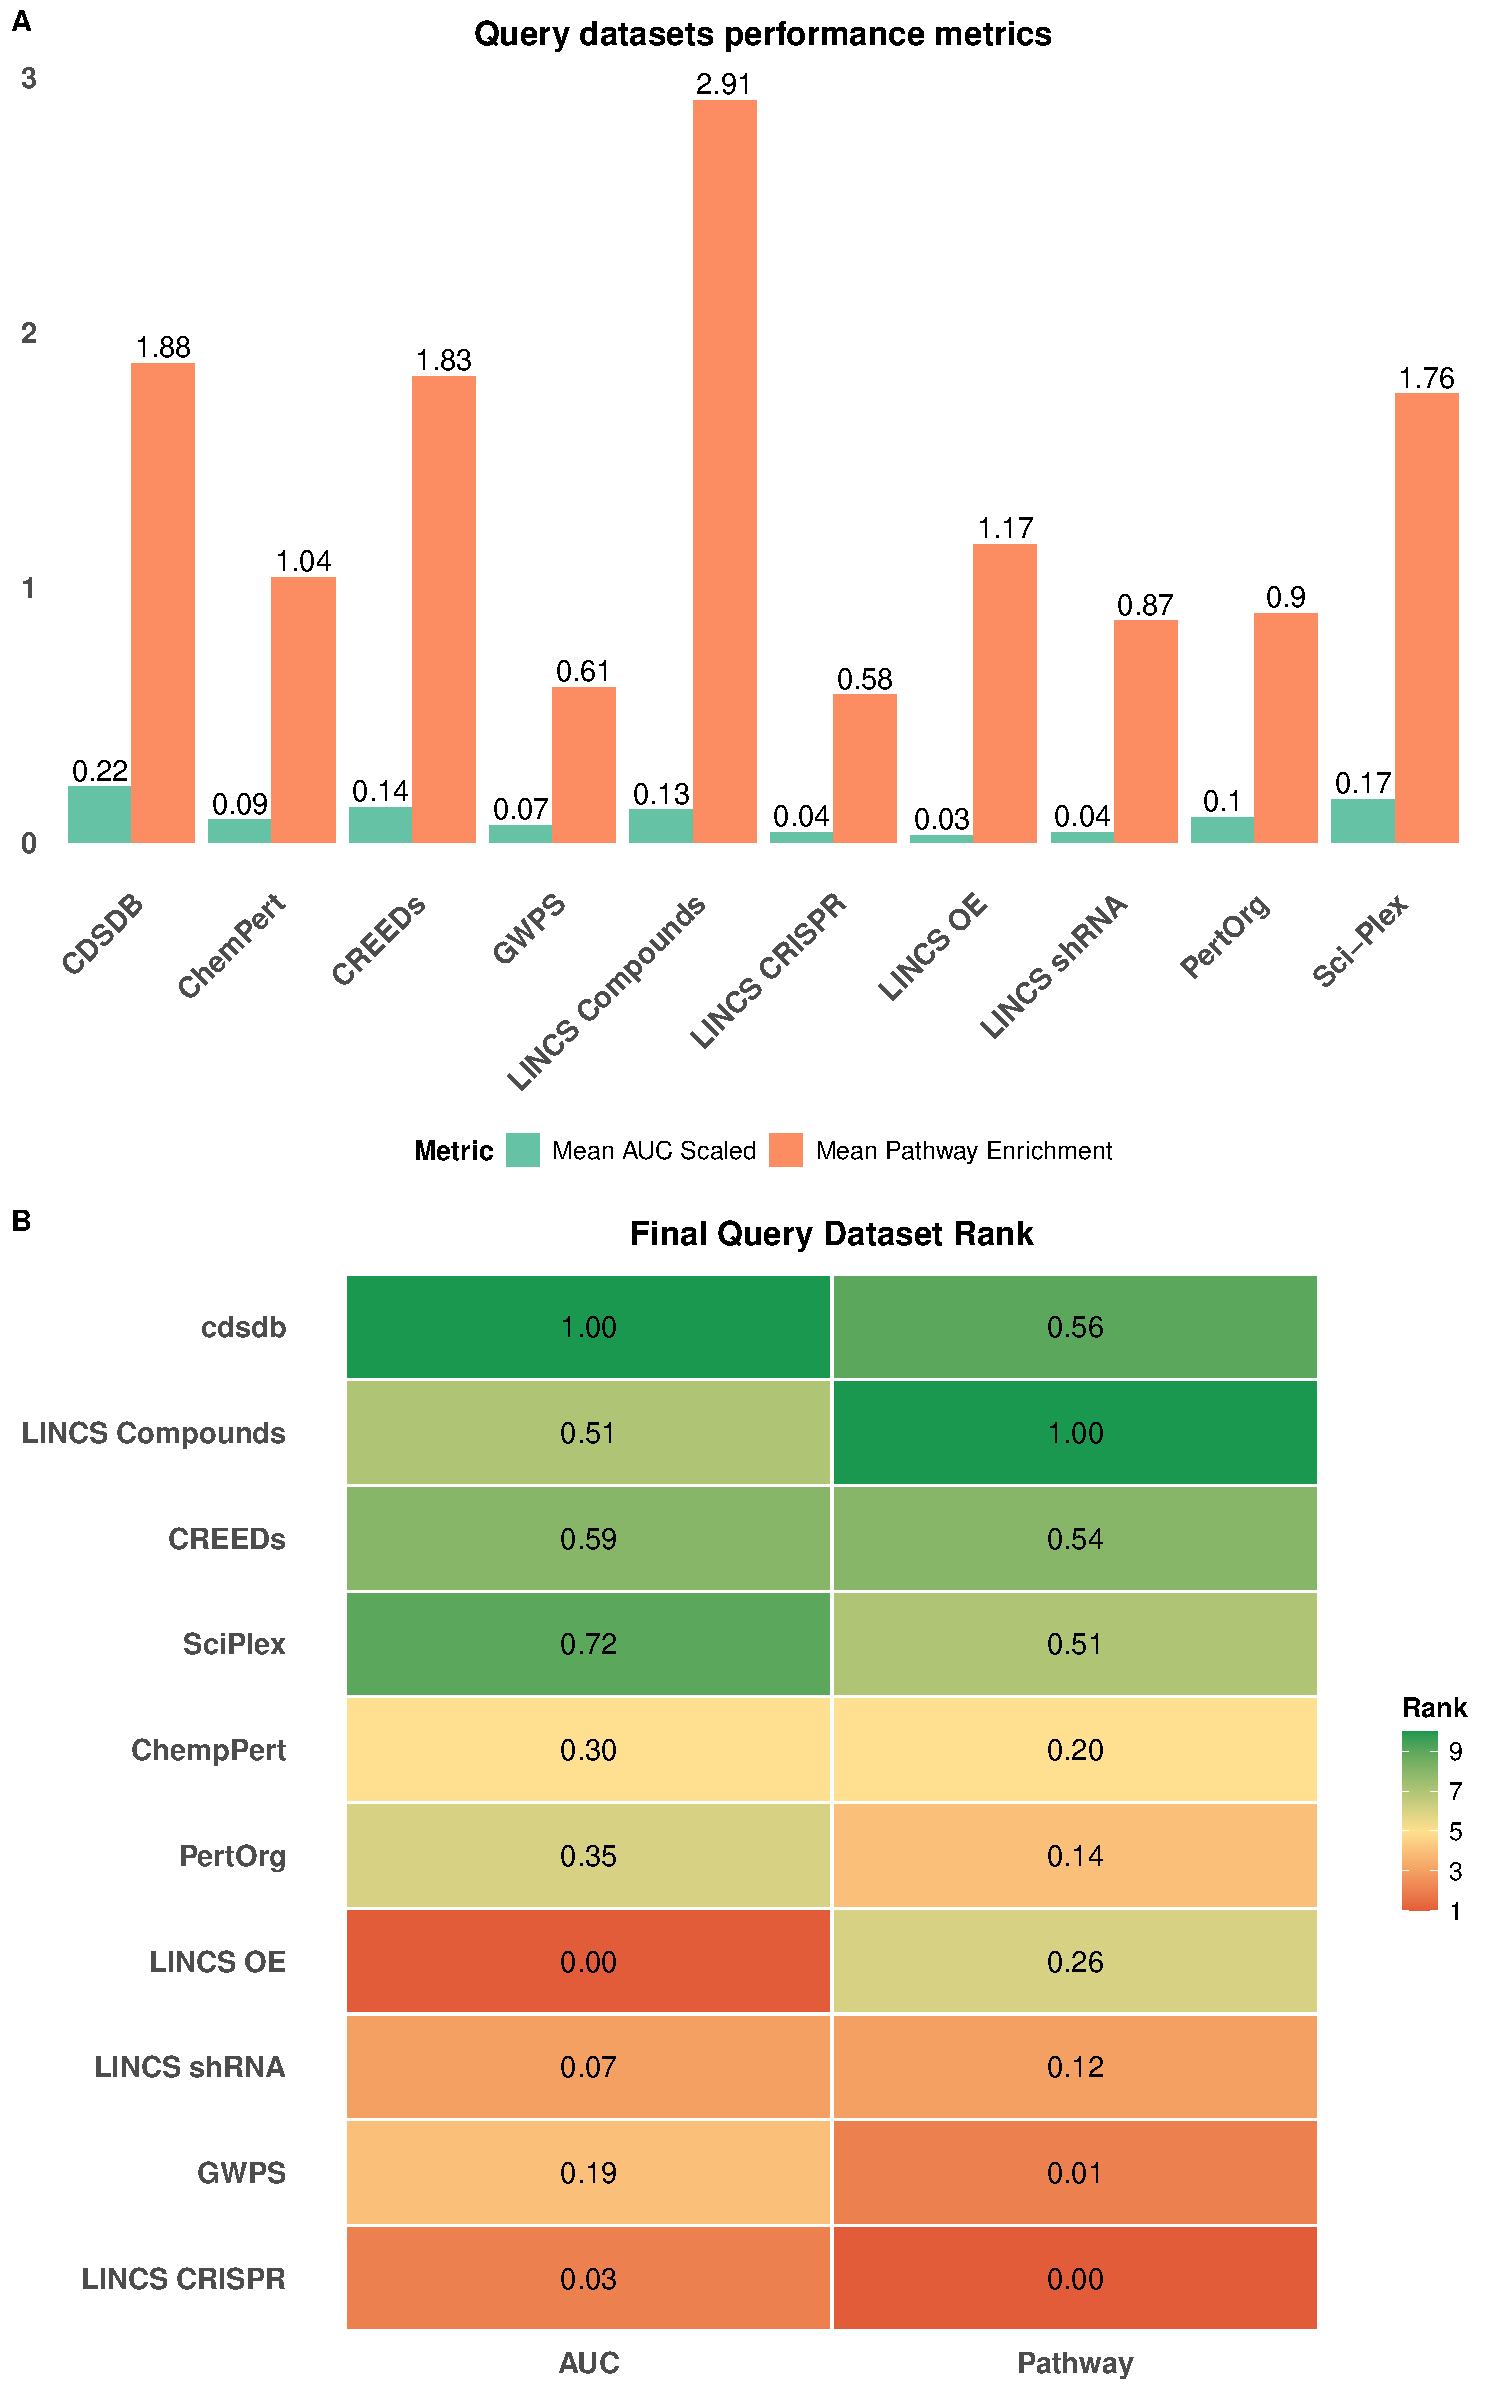
\includegraphics[height=6in]{fig4.3.querywrapplots}
    \caption[Query dataset performance evaluation.]{Query dataset performance evaluation. A. Bar plot displaying performance metrics (\gls{AUC} and pathway enrichment scores) for each query dataset, with values shown above bars. B. Heatmap visualization of query dataset rankings based on AUC and pathway enrichment performance, ordered by final aggregate rank from lowest (bottom) to highest (top). Cell values represent normalized scores (0-1 scale) while color intensity indicates rank position, with green representing better performance. Query datasets include both drug and genetic perturbation experiments from various sources including cell lines, tissues, and single-cell platforms.}
    \label{fig:fig4.3.querywrapplots}
\end{figure}
%\end{newpdflayout}

\gls{CDS-DB}, a drug perturbation dataset derived entirely from cancer patient samples, obtained the highest overall performance with \gls{AUC} and pathway enrichment scores of 1.00 and 0.56, respectively. \gls{CDS-DB}, \gls{CREEDS}, and PertOrg, some of the top-performing datasets, represent tissue or \textit{in vivo} samples. Signatures from collected samples may be better for regulatory inference compared to cell-line models, as cell lines often accumulate individual and cluster of mutations often not detected in clinical patients, as the result ex-vivo expansion. This pattern is also visible when comparing by grouping tissue versus cell-line (Figure~\ref{fig:fig4.3.allcomparisonsfacetednorank}). The tissue versus cell-line comparison showed better \gls{AUC} for tissue-derived signatures, aligning with the individual dataset observations. The drug versus genetic perturbation comparison also revealed a pattern. Algorithms consistently performed better on drug perturbation datasets. This distinction is evident from most algorithms falling below the diagonal line for \gls{AUC}. Drug perturbations apparently are more reliable signatures for target recovery across diverse algorithmic approaches. This is even more pronounced individually (Figure~\ref{fig:fig4.3.querywrapplots}) for \gls{LINCS}, which comes from the same platform. \gls{LINCS} Compounds ranked second overall with the best mean pathway enrichment value. On the other hand, genetic perturbations from the same \gls{LINCS} platform (\gls{CRISPR}, shRNA, and \gls{OE}) showed poor target recovery with \gls{AUC} values between 0.03 and 0.04, with \gls{LINCS} \gls{CRISPR} obtaining the last position in the rank. 
The bulk versus single-cell comparison revealed no specific differences, with algorithms grouping evenly around the diagonal in Figure~\ref{fig:fig4.3.allcomparisonsfacetednorank}. Looking at individual single-cell datasets, Sci-Plex (\gls{AUC} score: 0.72; Pathway enrichment score: 0.51) performed far better than \gls{GWPS} (\gls{AUC} score: 0.19; Pathway enrichment score: 0.01). The similar performance of single-cell and bulk query datasets and the inconsistent results obtained with the latter may suggest that the sequencing technology by itself is not the factor most responsible for the variability of algorithm performance.

\begin{figure}[htbp]
    \centering
    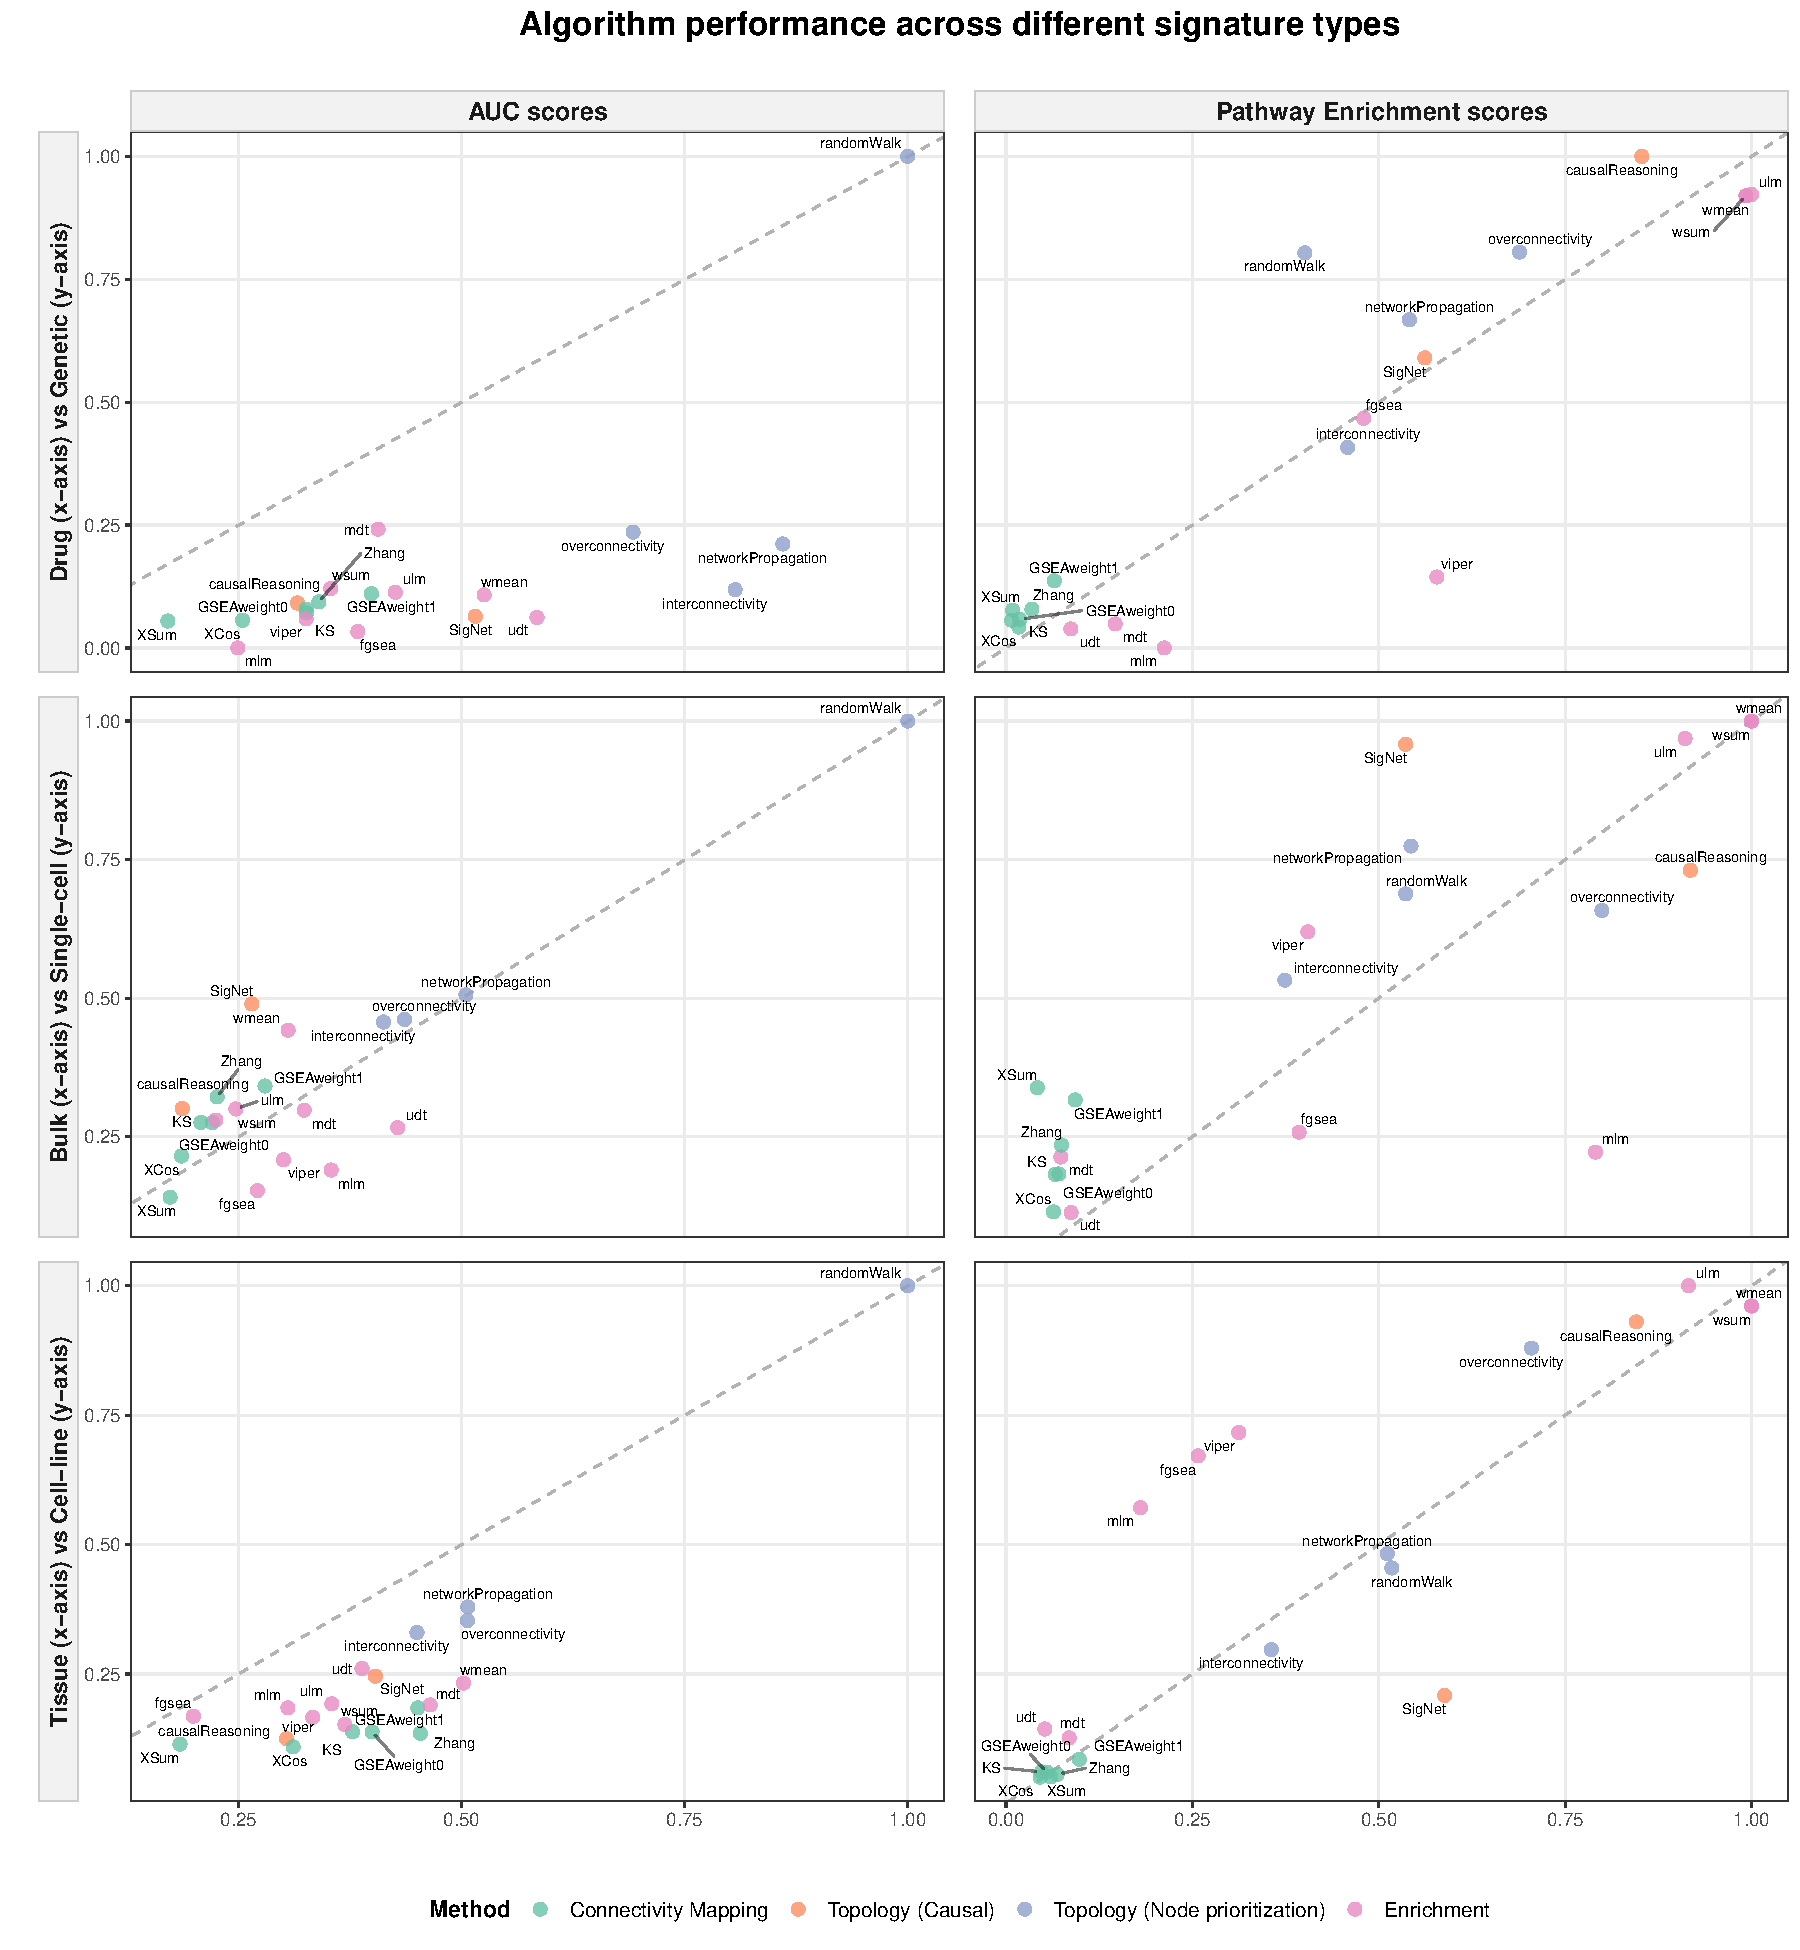
\includegraphics[height=5.5in]{fig4.3.allcomparisonsfacetednorank}
    \caption[Comparison of algorithm performance between different signature types.]{Comparison of algorithm performance between different signature types, across two evaluation metrics (\gls{AUC} scores and Pathway Enrichment scores). Different comparison: drug perturbation vs genetic perturbation signatures (top), bulk \gls{RNA-seq} vs \gls{scRNA-seq} data (middle), and tissue-derived vs cell-line-derived signatures (bottom). Each dot represents an algorithm, colored by category. The diagonal dashed line indicates equal performance between the two signature types being compared. Dots above the line indicate better performance on the y-axis signature type, while dots below the line indicate better performance on the x-axis signature type.}
    \label{fig:fig4.3.allcomparisonsfacetednorank}
\end{figure}
%\end{newpdflayout}


